\section{PID pozíció szabályozás szimmetrikus optimum módszerrel}

%{{{ P, I és D paraméterek számítása
\subsection{P, I és D paraméterek számítása}

Az előző feladatból a szabályzót változtassuk meg egy PID kontrollerre:
\begin{equation}
	\fn{W}_\text{c} = P\frac{(1+T_\text{I}s)(1+T_\text{D}s)}{s(1+nT_\text{D})}.
\end{equation}
Válasszuk meg a deriváló tag időállandóját úgy, hogy az kiejtse a szabályozott szakasz
egyik pólusát, tehát legyen $T_\text{D} = T_2$.

Írjuk fel az előrevezető ág átviteli függvényét:
\begin{equation}
	\fn{W}_\text{x} = \fn{W}_\text{c}\fn{W}_\text{p}\frac{1}{s} = 
	\frac{P}{s^2}\frac{(1+T_\text{I}s)\bcancel{(1 + T_\text{D}s)}}{1 + nT_\text{D}s}\frac{\Psi}{(1 + sT_1)\bcancel{(1 + sT_2)}}
\end{equation}
ahol $\Psi$ a szabályozott szakasz erősítése.

Ezután írjuk fel a fázistolást a körfrekvencia függvényében:
\begin{equation}
	\varphi(\omega) = -\pi - \operatorname{arctg}(T_1\omega) - \operatorname{arctg}(nT_\text{D}\omega) + \operatorname{arctg}(T_\text{I}\omega).
\end{equation}
Ennek a függvénynek a szélsőértékét keressük. Ehhez tegyük nullává a deriváltat:
\begin{equation}
	\frac{\partial\varphi}{\partial\omega} = 
	\frac{T_\text{I}}{\brc{T_\text{I}\omega}^2+1} - 
	\frac{nT_\text{D}}{\brc{T_\text{D}\omega}^2+1} - 
	\frac{T_\text{1}}{\brc{T_\text{1}\omega}^2+1} = 0.
\end{equation}
Ebből megkaptunk egy $\omega_\text{c}$ értéket, ami $T_\text{I}$-től függ.
Ezt helyettesítsük be a fázistartalékhoz tartozó képletbe, ami kiadja $T_\text{D}$-t és
ezáltal $\omega_\text{c}$ numerikus értékét is:
\begin{equation}
	\varphi_\text{t} = \pi + \varphi(\omega_\text{c}).
\end{equation}
Ebből $T_\text{I} = 0,2022$ s, és $\omega_\text{c} = 18,4589~\frac{\text{rad}}{\text{s}}$.

Már csak a $P$ körerősítést kell meghatároznunk, ami ugyanúgy történik mint az első feladatban:
\begin{equation}
	\abs{\fn{W}_\text{x}(\omega_\text{c})} = 1 \Rightarrow P = 1,0747.
\end{equation}

Ellenőrizzük, hogy a fázistartalék tényleg $60^\circ$-e a \verb|margin| függvénnyel.
\begin{figure}[H]
	\centering
	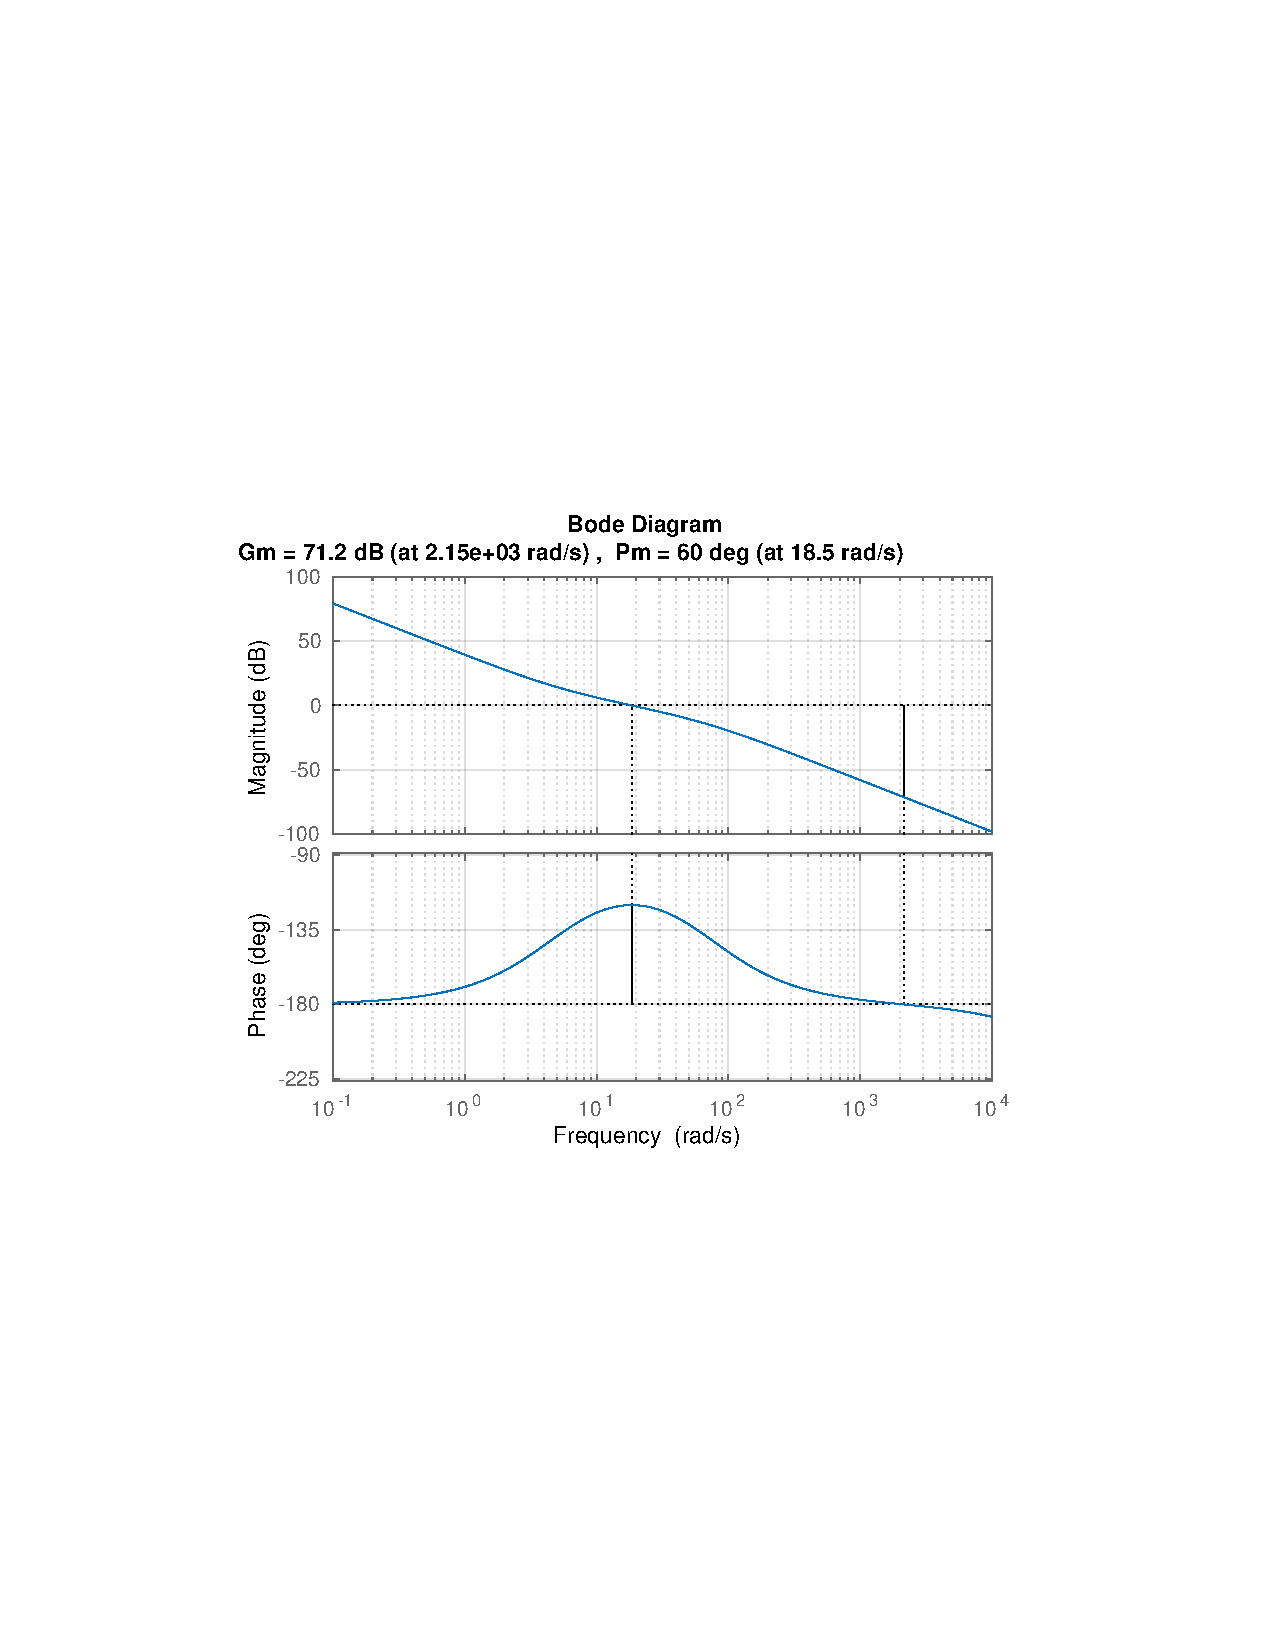
\includegraphics[width=.7\textwidth, trim=100 240 80 246, clip]{4a_margin}
	\caption{PID pozíció-szabályzott rendszer Bode-diagramja, fázistartalék feltüntetve}
	\label{fig:4a_margin}
\end{figure}

Ez teljesül.

%}}}

%{{{ Egységugrás válasz
\subsection{Egységugrás válasz}

Egy kör fordulat szabályozása esetén a bemenet Laplace-transzformáltja $\fn{X}=\frac{2\pi}{s}$,
a kimenet ebből $\fn{Y} = \fn{W}_\text{cl}\fn{X}$. Ezt a szokásos \verb|step| függvény
ki is rajzolja nekünk időtartományban, amit \aref{fig:4b_step}. ábra mutat.

\begin{figure}[H]
	\centering
	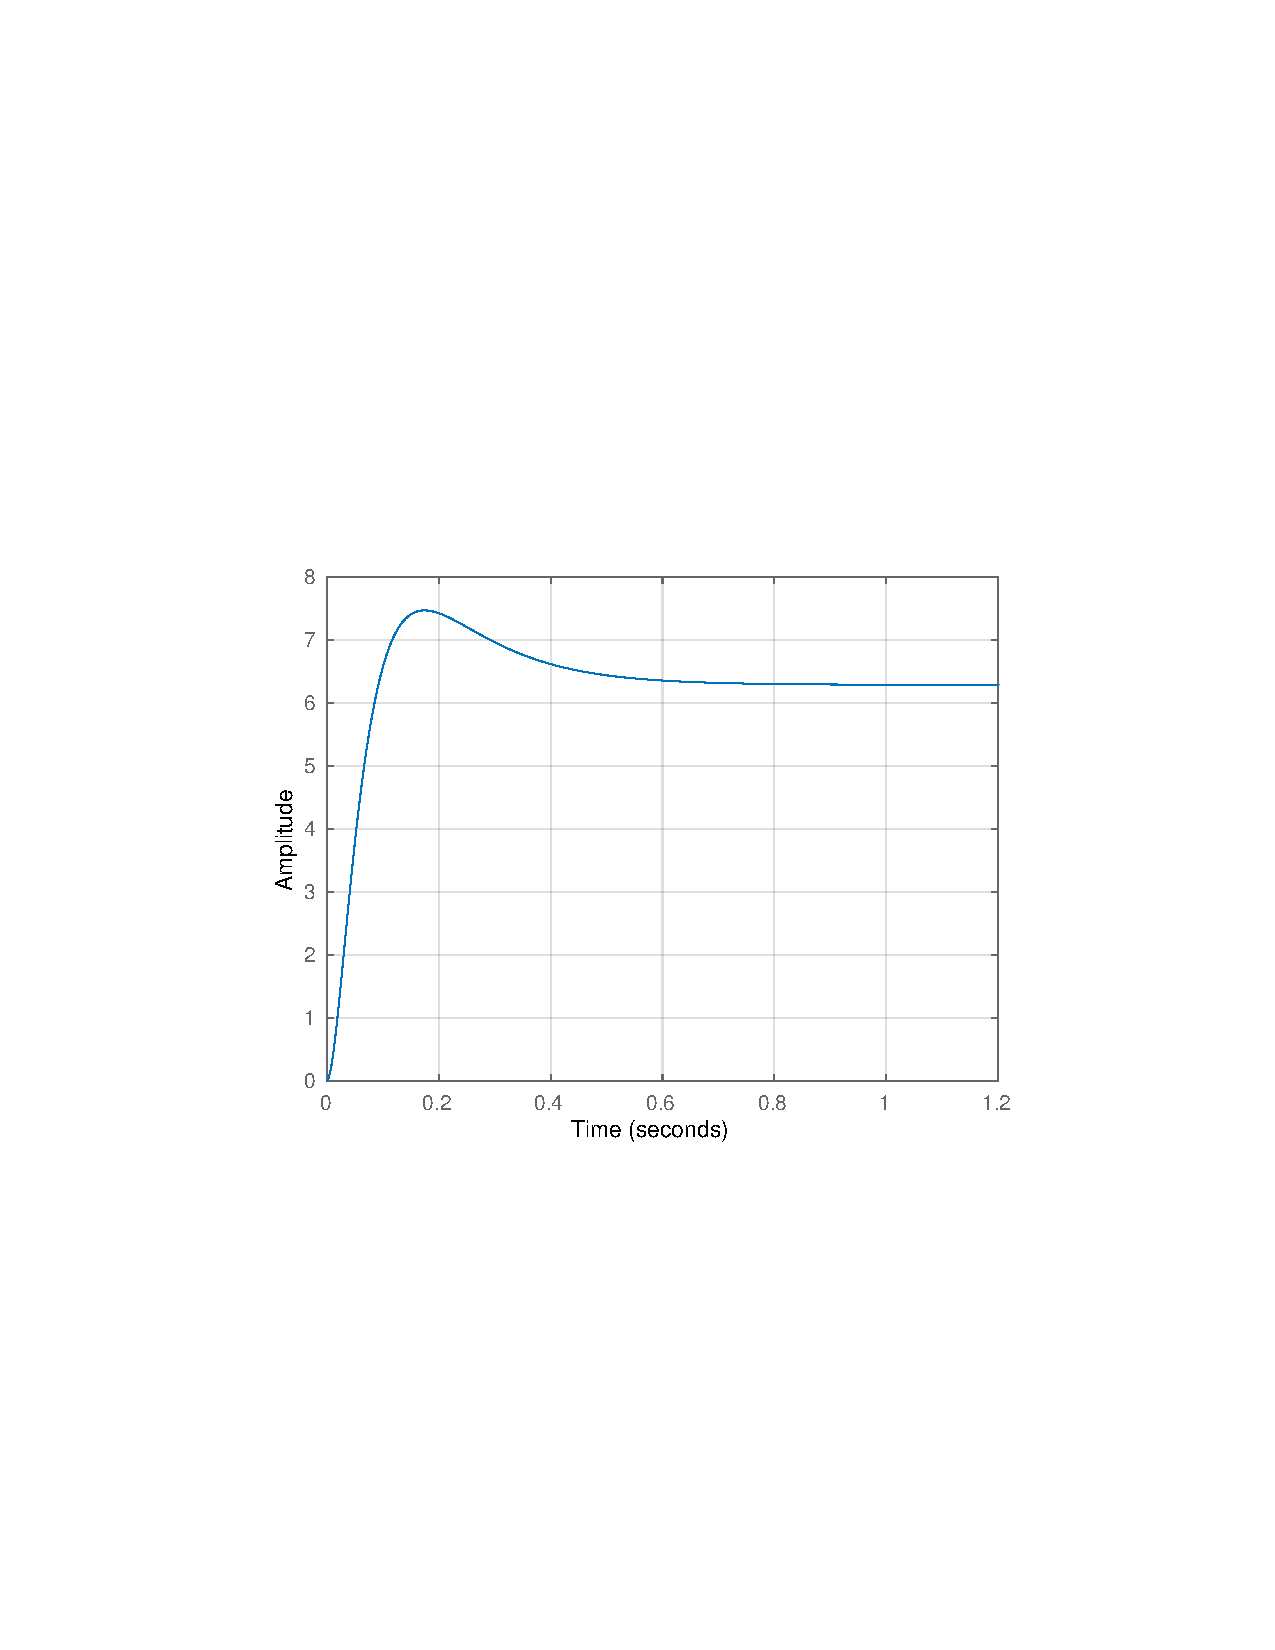
\includegraphics[width=.7\textwidth, trim=100 240 80 252, clip]{4b_step}
	\caption{PID egységugrás-válasz}
	\label{fig:4b_step}
\end{figure}

%}}}

%{{{ Állandósult szögsebesség
\subsection{Állandósult szögsebesség}

Az előző részfeladatban kiszámolt kimenetet felhasználva az állandósult szög érték:
$\theta_\infty = \lim\limits_{s\rightarrow 0}s\fn{Y} = 6,2832$ rad.

Az állandósult hiba a PID szabályzótól vártan zérus.

%}}}
